\documentclass[10.5pt,a4paper]{article}
\usepackage[margin=2.3cm,top=2.6cm,bottom=2.4cm]{geometry}
\usepackage{fontspec}
\setmainfont{Inter-Regular.ttf}[Path=../fonts/,BoldFont=Inter-SemiBold.ttf,ItalicFont=Inter-Italic.ttf]
\newfontfamily\titlefont{SpaceGrotesk-Bold.ttf}[Path=../fonts/]
\setmonofont{IBMPlexMono-Regular.ttf}[Path=../fonts/,Scale=0.88]
\usepackage{amsmath,amssymb}
\usepackage{float}\usepackage{xcolor,tikz,graphicx,booktabs,enumitem,tcolorbox,fancyhdr,titlesec,caption,array,microtype,siunitx}
\usetikzlibrary{calc}
\tcbuselibrary{skins}
\sisetup{per-mode=symbol}
\definecolor{ink}{HTML}{1A1A1A}\definecolor{dark}{HTML}{14261C}\definecolor{amber}{HTML}{E8A13A}\definecolor{grn}{HTML}{1B3A2B}\definecolor{mut}{HTML}{5C7A63}\definecolor{bone}{HTML}{F4F1EA}\definecolor{bonetwo}{HTML}{EDE8DC}\definecolor{sap}{HTML}{A9C7A0}
\definecolor{okbg}{HTML}{E1EBDB}\definecolor{badbg}{HTML}{F6E4C4}\definecolor{noteb}{HTML}{EDE8DC}
\color{ink}
\setlength{\parindent}{0pt}\setlength{\parskip}{6pt}\renewcommand{\arraystretch}{1.25}
\titleformat{\section}{\Large\bfseries\color{grn}}{\thesection}{0.7em}{}
\titleformat{\subsection}{\large\bfseries\color{grn}}{\thesubsection}{0.6em}{}
\titlespacing*{\section}{0pt}{16pt}{6pt}\titlespacing*{\subsection}{0pt}{12pt}{4pt}
\captionsetup{font={small},labelfont=bf,labelsep=period,justification=raggedright,singlelinecheck=false}
% Auselia mark: the brand SVGs converted to PDF (platform/brand/mark/svg), never redrawn
\newcommand{\lm}{
\includegraphics[height=0.85cm]{mark_color.pdf}}
\newcommand{\lmr}[1][1.25cm]{
\includegraphics[height=#1]{mark_reversed.pdf}}
\pagestyle{fancy}\fancyhf{}
\renewcommand{\headrulewidth}{0pt}
\newcommand{\faintmark}{\tikz[baseline=-0.9mm]\node[opacity=0.45,inner sep=0]{
\includegraphics[height=0.62cm]{mark_color.pdf}};}
\fancyfoot[L]{\faintmark\hspace{0.7em}{\ttfamily\fontsize{6.6}{8}\selectfont\color{mut}AUSELIA\ \ /\ \ AFE V1\ \ /\ \ BRING-UP GUIDE\ \ /\ \ VERSION 0.1}}
\fancyfoot[R]{{\ttfamily\fontsize{6.6}{8}\selectfont\color{mut}\thepage}}
\newenvironment{pass}{\begin{tcolorbox}[colback=okbg,colframe=grn,boxrule=0.5pt,arc=2pt,left=6pt,right=6pt,top=3pt,bottom=3pt,title={\textbf{Pass}},coltitle=white,fonttitle=\small,attach boxed title to top left={yshift=-2mm,xshift=2mm},boxed title style={colback=grn,arc=1pt}]}{\end{tcolorbox}}
\newenvironment{fail}{\begin{tcolorbox}[colback=badbg,colframe=amber!85!black,boxrule=0.5pt,arc=2pt,left=6pt,right=6pt,top=3pt,bottom=3pt,title={\textbf{If not}},coltitle=white,fonttitle=\small,attach boxed title to top left={yshift=-2mm,xshift=2mm},boxed title style={colback=amber!85!black,arc=1pt}]}{\end{tcolorbox}}
\newenvironment{warn}{\begin{tcolorbox}[colback=red!6,colframe=red!60!black,boxrule=0.6pt,arc=2pt,left=6pt,right=6pt,top=3pt,bottom=3pt,title={\textbf{Caution}},coltitle=white,fonttitle=\small,attach boxed title to top left={yshift=-2mm,xshift=2mm},boxed title style={colback=red!60!black,arc=1pt}]}{\end{tcolorbox}}
\newcommand{\stepno}[2]{\vspace{4pt}\noindent\tikz[baseline=(n.base)]{\node[fill=grn,text=white,rounded corners=2pt,inner sep=4pt,font=\bfseries\small] (n) {STEP #1};}\hspace{0.6em}{\Large\bfseries #2}\par\vspace{2pt}}
\newcommand{\goal}[1]{{\color{mut}\emph{Goal: #1}}\par}
\newcommand{\tp}[1]{\texttt{TP#1}}
\setlist[enumerate]{leftmargin=2em,itemsep=2pt,topsep=2pt}
\setlist[itemize]{leftmargin=1.4em,itemsep=2pt,topsep=2pt}
\begin{document}
% ---------------- cover (white, printer friendly: mark with signal rings, wordmark above the title)
\thispagestyle{empty}
\begin{tikzpicture}[remember picture,overlay]
 \pgfmathsetmacro{\H}{9.4}\pgfmathsetmacro{\sc}{\H/64}
 \node[anchor=north east,inner sep=0] (m) at ($(current page.north east)+(-1.6cm,-2.6cm)$) {
\includegraphics[height=\H cm]{mark_color.pdf}};
 \coordinate (c) at ($(m.north west)+(32.6*\sc cm,-21*\sc cm)$);
 \draw[amber,opacity=0.75,line width=0.5pt] (c) circle (11.1*\sc cm);
 \draw[amber,opacity=0.5,line width=0.5pt] (c) circle (17.6*\sc cm);
 \draw[amber,opacity=0.32,line width=0.5pt] (c) circle (27.9*\sc cm);
 \node[anchor=north west,xshift=2.2cm,yshift=-2.6cm,font=\scriptsize\ttfamily,text=mut] at (current page.north west) {BRING-UP GUIDE\ \ /\ \ VERSION 0.1};
 \node[anchor=north west,xshift=2.2cm,yshift=-13.3cm] at (current page.north west) {\titlefont\fontsize{46}{46}\selectfont\color{grn}AUS\color{amber}ELIA};
 \node[anchor=north west,text width=15.5cm,xshift=2.2cm,yshift=-15.4cm] at (current page.north west) {\titlefont\fontsize{26}{31}\selectfont\color{grn}Analog Front-End (AFE) v1:\\bring-up guide};
 \node[anchor=north west,text width=15cm,xshift=2.2cm,yshift=-19.0cm] at (current page.north west) {\large\color{ink} From the first look at the board to the sensor on the plant.};
 \node[anchor=north west,text width=14cm,xshift=2.2cm,yshift=-21.2cm] at (current page.north west) {\small\color{mut} Each step has a goal, a list of actions, a table of expected values, and a check list for a wrong result. The simulation of the as-built board gives each expected value.};
 \node[anchor=north west,xshift=2.2cm,yshift=-25.2cm,font=\scriptsize\ttfamily,text=mut] at (current page.north west) {Version 0.1\ \ /\ \ November 4, 2026\ \ /\ \ Nicol\'as Villegas};
 \node[anchor=north west,xshift=2.2cm,yshift=-27.6cm,font=\tiny\ttfamily,text=mut] at (current page.north west) {AUSELIA\ \ /\ \ AFE V1\ \ /\ \ BRING-UP GUIDE\ \ /\ \ VERSION 0.1};
\end{tikzpicture}
\clearpage
% ---------------- 1
\section{About this guide}
This guide takes the first AFE boards from the box to a measured result. The steps follow the signal. First, apply power. Then test the chain, the listener, and the SPI (serial peripheral interface) link. Last, test the sensor head and put it on the plant.

Each step has the same parts: a goal, a list of actions, a table of expected values, a green Pass box, and an amber If-not box. The simulation of the as-built netlist gives the expected values. No real board has given a measurement yet. Your readings are the first.

\begin{figure}[H]
\centering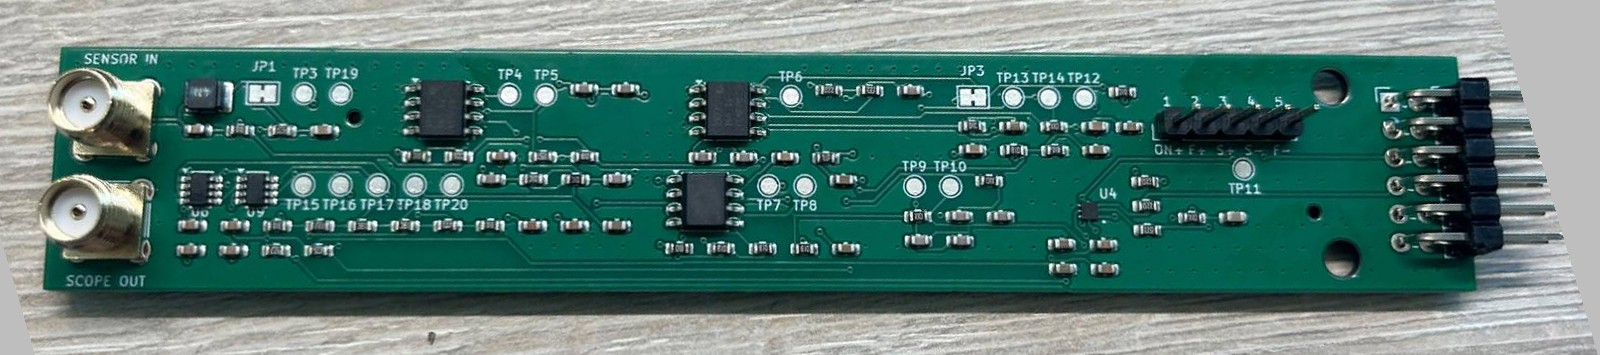
\includegraphics[width=\textwidth]{board_photo.jpg}
\caption{The AFE v1 test board, top side. SENSOR IN (J1) and SCOPE OUT (J4) are on the left. The power header J7 and the PMOD (peripheral module connector) J3 are on the right.}
\end{figure}

\subsection{What you need}
\begin{tabular}{@{}p{5.4cm}p{9.2cm}@{}}
\toprule Item & Use\\\midrule
Keysight B2901BL source-measure unit (SMU) & Supplies power through J7 and measures the supply current with four wires\\
Function generator or Analog Discovery 2 & Makes bursts of 10 cycles at 250 kHz from a 50 $\Omega$ output\\
Oscilloscope, 250 MS/s or faster & Measures the test points with a 1 M$\Omega$ input\\
Multimeter & Measures resistance and DC voltage\\
ZedBoard with a program that reads the ADC & Runs the SPI link and reads the listener lines (Steps 6 and 7)\\
10 pF and 1600 pF C0G capacitors & Inject charge and replace the sensor\\
SMA cables, a jumper for J7, a knife, a soldering iron & Cut and close JP1 and JP3\\
Magnifier or microscope & Examines U4, U6, and U9\\
\bottomrule\end{tabular}

\clearpage
\subsection{Test setup}
Figure~\ref{fig:setup} shows the setup for the signal tests in Steps 3 to 5.
\begin{figure}[H]
\centering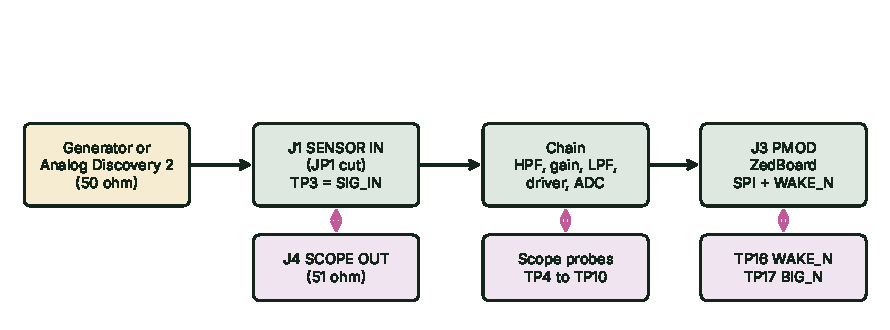
\includegraphics[width=0.92\textwidth]{fig_setup.pdf}
\caption{Test setup for Steps 3 to 5.}\label{fig:setup}
\end{figure}

\begin{warn}
Cut JP1 before you connect a generator to J1. The center pin of J1 carries 3.3 V DC when JP1 is closed. The generator would receive this voltage. Cut JP1 with a knife for Steps 3 to 5. Close JP1 again with solder for Steps 8 to 10.\\[3pt]
Touch a grounded surface before you touch the board. The ADC U4 and the comparators U6 and U9 are small parts with a fine pitch.
\end{warn}

% ---------------- 2
\clearpage
\section{Know the board}
Figure~\ref{fig:map} shows each part and each test point (TP). The red dot on an IC marks pin 1. Table~\ref{tab:tp} lists each test point and the stage it measures.

\begin{figure}[H]
\centering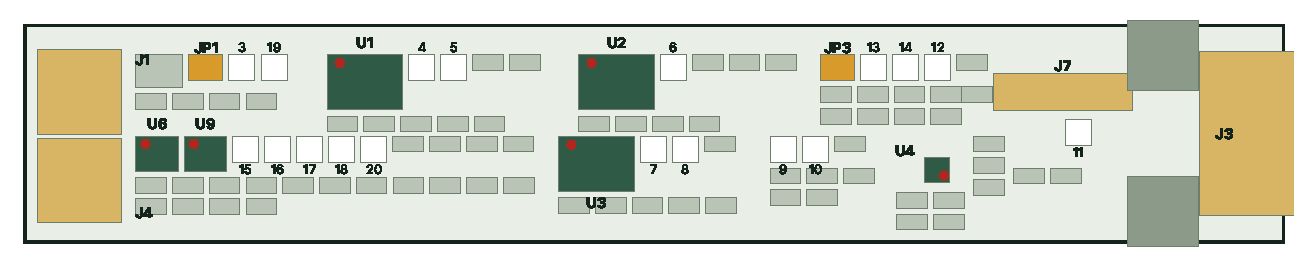
\includegraphics[width=\textwidth]{fig_boardmap.pdf}
\caption{Top view with each part. Green: ICs with a red pin 1 dot. Gold: connectors. Orange: solder jumpers JP1 and JP3. White: test points, shown by number.}\label{fig:map}
\end{figure}

\begin{table}[H]
\caption{Test points of the main board. SIG\_IN is the input after the bias-T.}\label{tab:tp}
\small\begin{tabular}{@{}lll@{\hspace{1.2em}}lll@{}}
\toprule TP & Net & Shows & TP & Net & Shows\\\midrule
\tp{3} & SIG\_IN & input & \tp{12} & AVDD & ADC reference\\
\tp{4} & HPF\_OUT & high-pass filter & \tp{13} & VMID5 & 1.65 V mid-rail\\
\tp{5} & GAIN\_OUT & gain stage & \tp{14} & VOCM & driver center\\
\tp{6} & LPF\_OUT & low-pass filter & \tp{15} & LST & listener signal\\
\tp{7} & DRV\_OUTP & driver $+$ & \tp{16} & WAKE\_N & small window\\
\tp{8} & DRV\_OUTN & driver $-$ & \tp{17} & BIG\_N & large window\\
\tp{9} & AINP & ADC input $+$ & \tp{18} & REFL & listener center\\
\tp{10} & AINM & ADC input $-$ & \tp{19}, \tp{20} & GND & scope ground\\
\tp{11} & +3V3 & board rail & & &\\
\bottomrule\end{tabular}
\end{table}

\subsection{The signal path}
Figure~\ref{fig:ladder} shows the signal size at each test point for a sine at 250 kHz. The gain of the chain to the ADC is about 4.1. The driver divides the signal into two halves of opposite sign around 1.65 V.
\begin{figure}[H]
\centering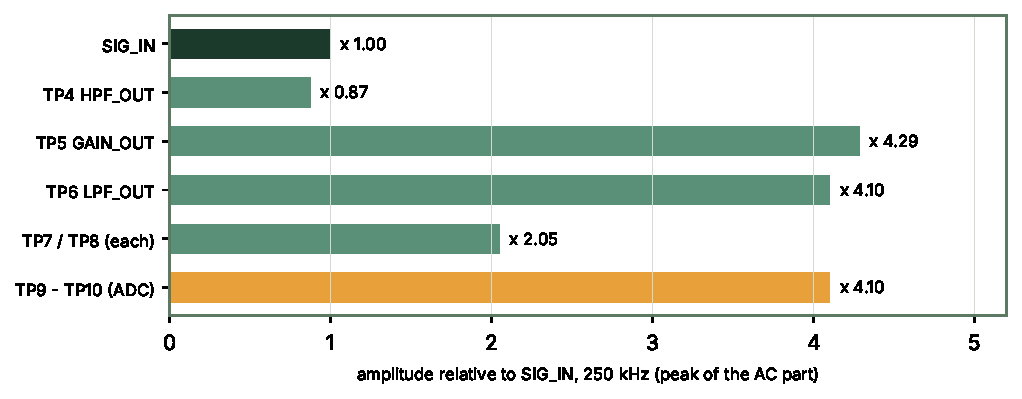
\includegraphics[width=0.92\textwidth]{fig_ladder.pdf}
\caption{Expected amplitude at each test point at 250 kHz, relative to SIG\_IN (ngspice, as-built netlist).}\label{fig:ladder}
\end{figure}

% ---------------- Step 0
\clearpage
\begin{samepage}
\stepno{0}{Look first, with the power off}
\goal{find a wrong part, a short, or a solder bridge before current flows.}
\begin{enumerate}
\item Examine the top side with the magnifier.
\item Compare the board with Figure~\ref{fig:map} and with the photo on page 2.
\item Make sure pin 1 of each IC is at the correct end. Use Table~\ref{tab:pin1}.
\item Examine U4, U6, and U9 for solder bridges between pads.
\item Make sure the pins of J3 and J7 are straight.
\item Make sure J3 is flush with the board edge.
\item Measure the resistance from \tp{11} (+3V3) to \tp{19} (GND). Wait until the value is stable.
\end{enumerate}
\begin{table}[H]
\caption{Pin 1 positions. View from the top, with SENSOR IN on the left.}\label{tab:pin1}
\small\begin{tabular}{@{}lllp{6.6cm}@{}}
\toprule Ref & Part & Package & Pin 1\\\midrule
U1, U2, U3 & OPA2365, OPA2365, THS4531 & SOIC-8 & top left, next to the silkscreen triangle\\
U4 & ADS7057 & X2QFN-8 & lower right of the part\\
U6, U9 & TLV7022 & SOT-23-8 & top left\\
U8 (head) & OPA365 & SOT-23-5 & lower pin on the right side, next to the silkscreen triangle\\
\bottomrule\end{tabular}
\end{table}
\begin{pass}
The resistance is about 2 k$\Omega$. This is an estimate: the VOCM divider (2 k$\Omega$), the VMID5 divider (20 k$\Omega$), and the ladder (2.1 M$\Omega$) are in parallel. Any value above 1 k$\Omega$ is correct. No bridges are visible. Each pin 1 agrees with Table~\ref{tab:pin1}.
\end{pass}
\begin{fail}
If the resistance is below 500 $\Omega$, there is a short. Do not apply power. Look for a bridge at U4, U6, or U9. Look for a turned IC or a bridged C0G capacitor. A value that rises slowly is only the capacitors that charge.
\end{fail}
\end{samepage}

% ---------------- Step 1
\clearpage
\begin{samepage}
\stepno{1}{Power up with the SMU}
\goal{make sure the board uses the correct current and each rail has its value.}
J7 is the power entry. Do not connect the ZedBoard in this step.
\begin{figure}[H]
\centering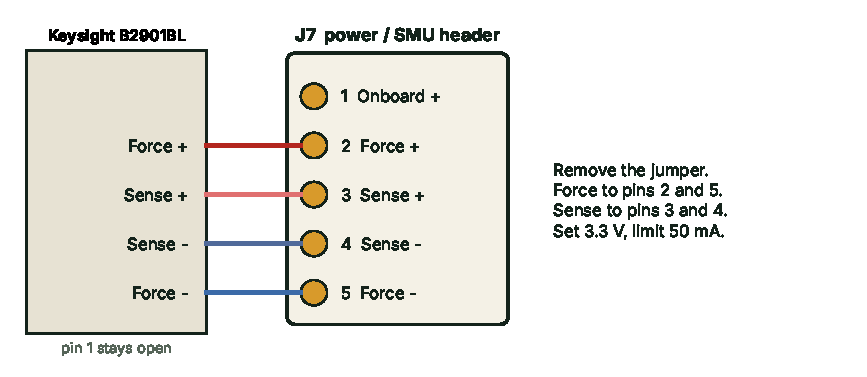
\includegraphics[width=0.78\textwidth]{fig_j7_smu.pdf}
\caption{Four-wire connection of the B2901BL to J7. Pins 2 and 3 meet at the board rail. Pins 4 and 5 are ground.}
\end{figure}
\begin{enumerate}
\item Remove the jumper from J7. Do not connect the PMOD. Leave JP1 closed.
\item Set the SMU to voltage source mode. Set the voltage to 3.3 V. Set the current limit to 50 mA. Turn remote sense on. Keep the output off.
\item Connect Force to pins 2 and 5 of J7. Connect Sense to pins 3 and 4.
\end{enumerate}
\begin{warn}
Turn the output off if the current is more than 60 mA. This prevents damage to the board.
\end{warn}
\begin{enumerate}[resume]
\item Turn the output on. Read the current after one second.
\item Measure each node in Table~\ref{tab:dc} against GND (\tp{19}).
\end{enumerate}
\begin{table}[H]
\caption{Expected DC values (ngspice, all links closed, head not connected). The tolerance is $\pm$30 mV for 3.3 V nodes and $\pm$50 mV for other nodes.}\label{tab:dc}
\small\begin{tabular}{@{}lllp{5.8cm}@{}}
\toprule Node & Test point & Expected & Note\\\midrule
+3V3 & \tp{11} & 3.30 V & the SMU value\\
AVDD & \tp{12} & 3.27 V & after the 10 $\Omega$ and 10 $\mu$F filter\\
VMID5 & \tp{13} & 1.65 V & needs 25 ms after power-up\\
VOCM & \tp{14} & 1.64 V & half of AVDD\\
LST & \tp{15} & 1.64 V & rests at REFL\\
WAKE\_N, BIG\_N & \tp{16}, \tp{17} & 3.30 V & open drain with pull-up\\
REFL & \tp{18} & 1.64 V & middle of the ladder\\
Supply current & SMU & 20 to 22 mA & about 25 mA with the head\\
\bottomrule\end{tabular}
\end{table}
\begin{pass}The current is 18 to 30 mA. Each node agrees with Table~\ref{tab:dc}.\end{pass}
\begin{fail}
If the current is too high, turn the power off and do Step 2. If TP11 is low, check the Sense wires. If a mid-rail is wrong, wait 25 ms and measure again. Then check R7, R8, R14, and R15.
\end{fail}
\end{samepage}

% ---------------- Step 2
\clearpage
\begin{samepage}
\stepno{2}{Split the current with JP3}
\goal{find which part of the board uses the current.}
JP3 connects the capture rail to the 3.3 V rail. The capture rail supplies U1, U2, U3, and AVDD. The listener and DVDD are on the 3.3 V rail.
\begin{enumerate}
\item Turn the power off.
\item Cut JP3 with the knife.
\item Connect the SMU to the capture side of the gap, or put a second ammeter across the gap.
\item Measure the current of each side.
\item Close JP3 with a drop of solder.
\end{enumerate}
\begin{figure}[H]
\centering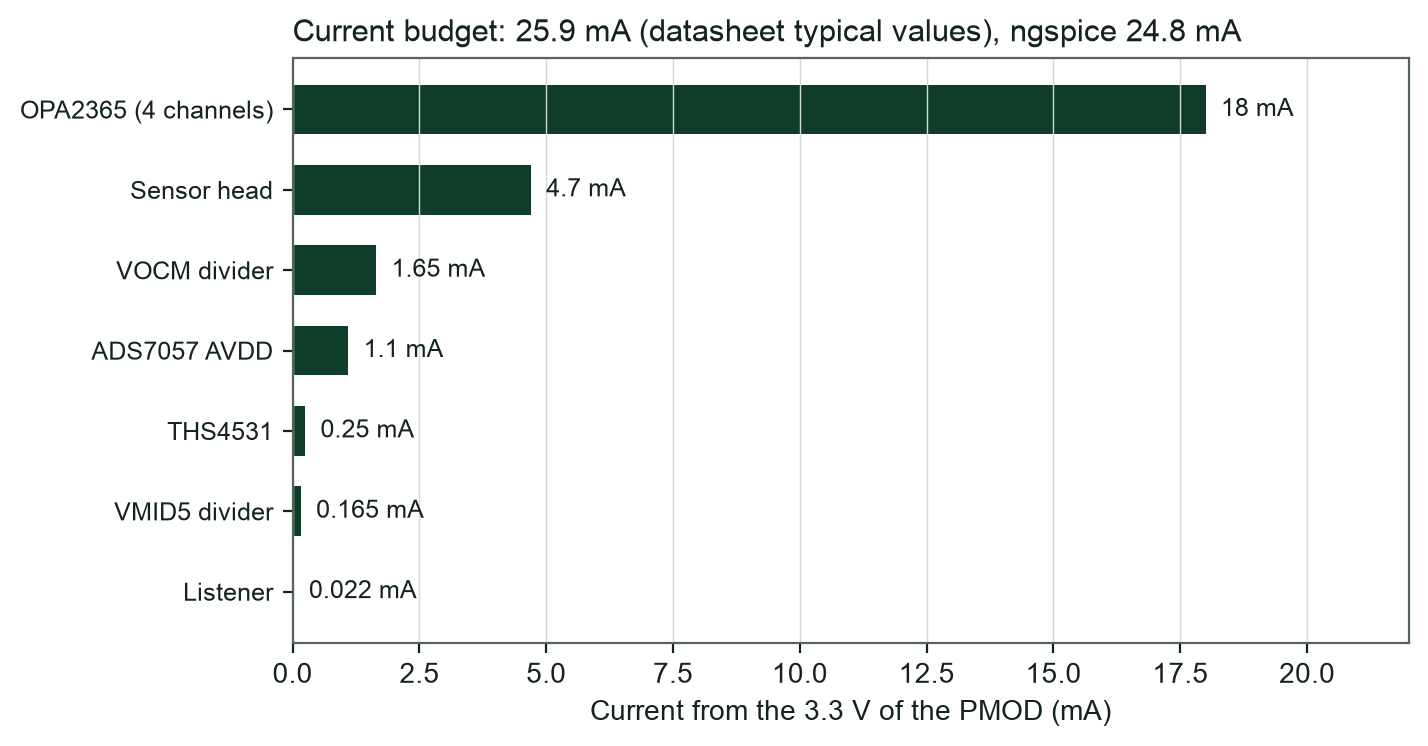
\includegraphics[width=0.56\textwidth]{fig_current.png}
\caption{Current budget (datasheet typical values, estimate). The four op-amp channels use the most current.}
\end{figure}
\begin{pass}The capture rail uses 20 to 22 mA. The other side uses about 0.3 mA.\end{pass}
\begin{fail}If the capture side is high, check U1, U2, U3, and the capacitors near them. If the other side is high, check U4, U6, and U9.\end{fail}
\end{samepage}

% ---------------- Step 3
\clearpage
\begin{samepage}
\stepno{3}{The signal chain at 250 kHz}
\goal{make sure each stage has the gain that the simulation gives.}
\begin{warn}Cut JP1 before you connect the generator. Keep the amplitude at SIG\_IN below 300 mV peak. A larger signal clips the gain stage.\end{warn}
\begin{enumerate}
\item Apply power as in Step 1.
\item Set the generator to a burst of 10 cycles at 250 kHz. Set the repeat time to 1 ms. Set the amplitude to 100 mV peak.
\item Connect the generator to J1.
\item Trigger the oscilloscope on \tp{3} (SIG\_IN).
\item Measure the peak of the AC part at each test point in Table~\ref{tab:gain}.
\item Look at \tp{7} and \tp{8}. Make sure they have opposite phase around 1.65 V (Figure~\ref{fig:waves}).
\item Measure SCOPE OUT (J4) with a 1 M$\Omega$ input. Make sure it agrees with \tp{6}.
\end{enumerate}
\begin{table}[H]
\caption{Expected peak at each test point for 100 mV peak at SIG\_IN and 250 kHz. The limit is $\pm$10\,\%.}\label{tab:gain}
\small\begin{tabular}{@{}llrp{5cm}@{}}
\toprule Test point & Net & Peak (mV) & Gain\\\midrule
\tp{3} & SIG\_IN & 100 & 1.00\\
\tp{4} & HPF\_OUT & 87 & 0.87\\
\tp{5} & GAIN\_OUT & 429 & 4.29\\
\tp{6} & LPF\_OUT & 410 & 4.10\\
\tp{7}, \tp{8} & DRV\_OUTP, DRV\_OUTN & $\pm$205 each & opposite signs around 1.65 V\\
\tp{9}, \tp{10} & AINP, AINM & $\pm$205 each & same as the driver\\
\tp{15} & LST & 68 & 0.68 (listener filter)\\
\bottomrule\end{tabular}
\end{table}
\begin{figure}[H]
\centering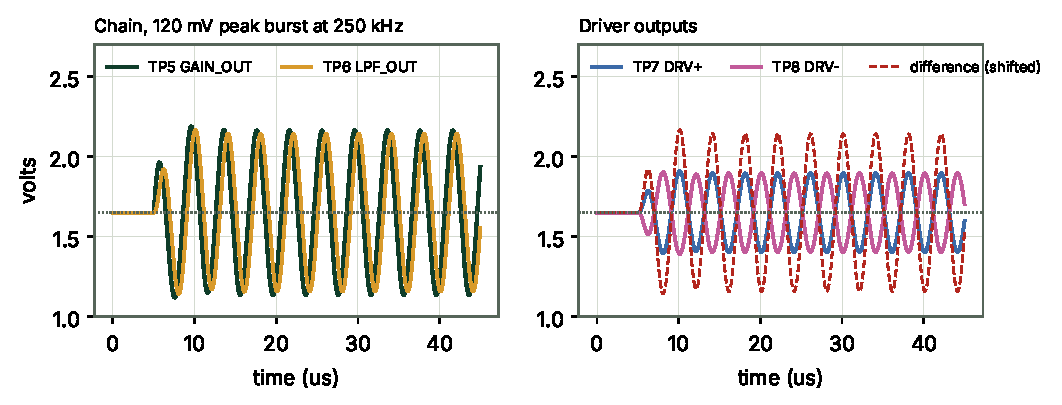
\includegraphics[width=0.86\textwidth]{fig_waves.pdf}
\caption{Expected waveforms for a burst of 120 mV peak (ngspice). The ADC measures the difference of TP7 and TP8.}\label{fig:waves}
\end{figure}
\begin{pass}Each peak is within 10\,\% of Table~\ref{tab:gain}.\end{pass}
\begin{fail}
Find the first stage that is wrong. If TP4 is wrong, check C1, C2, R1, R2, and pin 1 of U1. If TP5 is wrong, check R3 (3.9 k$\Omega$) and R4 (1 k$\Omega$). If TP6 is wrong, check R5, R6, and C4 to C6. If TP7 and TP8 are not opposite, check U3, R10 to R13, and VOCM at TP14.
\end{fail}
\end{samepage}

% ---------------- Step 4
\clearpage
\begin{samepage}
\stepno{4}{The frequency response}
\goal{make sure the band agrees with the simulation.}
\begin{enumerate}
\item Set the generator to a continuous sine of 100 mV peak.
\item Set the frequency to 10 kHz. Read the peak at \tp{6}.
\item Repeat for 30 kHz, 100 kHz, 250 kHz, 500 kHz, 1 MHz, and 2 MHz.
\item Calculate the gain of each frequency relative to 250 kHz, in dB.
\item Compare the result with Table~\ref{tab:sweep}.
\end{enumerate}
\begin{table}[H]
\caption{Expected response relative to 250 kHz (ngspice, whole chain to the ADC). The limit is $\pm$1.5 dB from 100 kHz to 500 kHz and $\pm$3 dB at other frequencies.}\label{tab:sweep}
\small\begin{tabular}{@{}lrrrrrrr@{}}
\toprule Frequency & 10 kHz & 30 kHz & 100 kHz & 250 kHz & 500 kHz & 1 MHz & 2 MHz\\\midrule
Gain (dB) & $-40.5$ & $-21.5$ & $-3.1$ & 0 & $-2.8$ & $-12.1$ & $-24.0$\\
\bottomrule\end{tabular}
\end{table}
\begin{pass}The result is within the limit of Table~\ref{tab:sweep} at each frequency.\end{pass}
\begin{fail}An error at the low end points to C1, C2, R1, or R2. An error at the high end points to C4, C5, C6, R5, or R6.\end{fail}
\end{samepage}

% ---------------- Step 5
\clearpage
\begin{samepage}
\stepno{5}{The listener: WAKE\_N and BIG\_N}
\goal{make sure the two window comparators fire near 35 mV and 111 mV at SIG\_IN.}
Keep the setup of Step 3, with JP1 cut. Probe \tp{15} (LST), \tp{16} (WAKE\_N), \tp{17} (BIG\_N), and \tp{18} (REFL).
\begin{enumerate}
\item Make sure \tp{18} reads 1.65 V.
\item Make sure \tp{16} and \tp{17} read 3.3 V with no signal.
\item Send the burst at 20 mV peak at SIG\_IN. Note the state of \tp{16} and \tp{17}.
\item Send the burst at 60 mV peak. Note the state of \tp{16} and \tp{17}.
\item Send the burst at 150 mV peak. Note the state of \tp{16} and \tp{17}.
\item To find the thresholds, increase the amplitude in steps of 5 mV. Note the amplitude when WAKE\_N falls and when BIG\_N falls.
\end{enumerate}
A line stays low only for the length of the burst.
\begin{table}[H]
\caption{Expected lines for a burst of 10 cycles at 250 kHz, with JP1 cut. The amplitude is the peak at SIG\_IN. Each threshold has a tolerance of $\pm$12 mV.}
\small\begin{tabular}{@{}rll@{}}
\toprule Amplitude & WAKE\_N (\tp{16}) & BIG\_N (\tp{17}) \\\midrule
20 mV & stays high & stays high\\
60 mV & falls & stays high\\
150 mV & falls & falls\\
\midrule Threshold & about 35 mV & about 111 mV\\
\bottomrule\end{tabular}
\end{table}
\begin{pass}Each line agrees with the table. Each threshold is within $\pm$12 mV. The response time is about 260 ns.\end{pass}
\begin{fail}If WAKE\_N is always low, make sure \tp{18} is 1.65 V. Then check R39 to R41, R21, and R23. If a threshold is far from the table, check R22, R41 (33 k$\Omega$), R39, and R40 (15 k$\Omega$). If no line falls, check U6, U9, R24, and R42.\end{fail}
\end{samepage}

% ---------------- Step 6
\clearpage
\begin{samepage}
\stepno{6}{The SPI link}
\goal{make sure the SPI frames are correct.}
The ZedBoard must run a program that drives CS and SCLK and reads SDO. Table~\ref{tab:pmod} gives the pins. The ADC only sends data, so the link has no MOSI line.
\subsection*{Power from the ZedBoard}
Do this part first. The SPI link needs the ZedBoard.
\begin{figure}[H]
\centering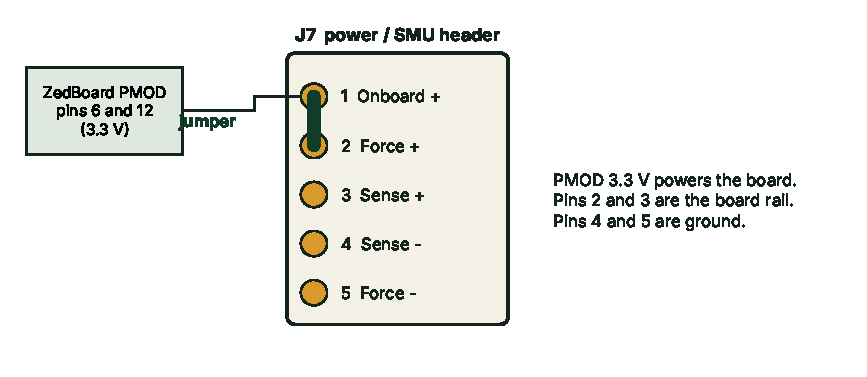
\includegraphics[width=0.36\textwidth]{fig_j7_pmod.pdf}
\caption{Power from the ZedBoard PMOD with a jumper on J7 pins 1 and 2.}
\end{figure}
\begin{enumerate}
\item Turn the power off.
\item Put the jumper on J7 pins 1 and 2.
\end{enumerate}
\begin{warn}Do not use the jumper and the SMU at the same time. The two sources would connect together.\end{warn}
\begin{enumerate}[resume]
\item Connect the board to a PMOD port of the ZedBoard.
\end{enumerate}
\end{samepage}
\clearpage
\begin{samepage}
\subsection*{Read the frames}
\textit{Step 6, continued.} Use the program on the ZedBoard.
\begin{table}[H]
\caption{Pins of the PMOD J3. The board uses nine of the twelve pins.}\label{tab:pmod}
\small\begin{tabular}{@{}rlrl@{}}
\toprule Pin & Signal & Pin & Signal\\\midrule
1 & CS & 7 & BIG\_N\\ 2 & not used & 8 & not used\\ 3 & SDO & 9 & not used\\ 4 & SCLK & 10 & WAKE\_N\\ 5 & GND & 11 & GND\\ 6 & 3V3 & 12 & 3V3\\
\bottomrule\end{tabular}
\end{table}
\begin{enumerate}
\item Apply no signal to J1. Set SCLK to 10 MHz.
\item Send one frame of 24 clocks. This frame calibrates the offset.
\item Send frames of 18 clocks.
\item Look at CS, SCLK, and SDO at the J3 pins. Compare them with Figure~\ref{fig:spi}.
\item Make sure the first frame returns zeros. Make sure each next frame returns the sample of the frame before.
\end{enumerate}
\begin{figure}[H]
\centering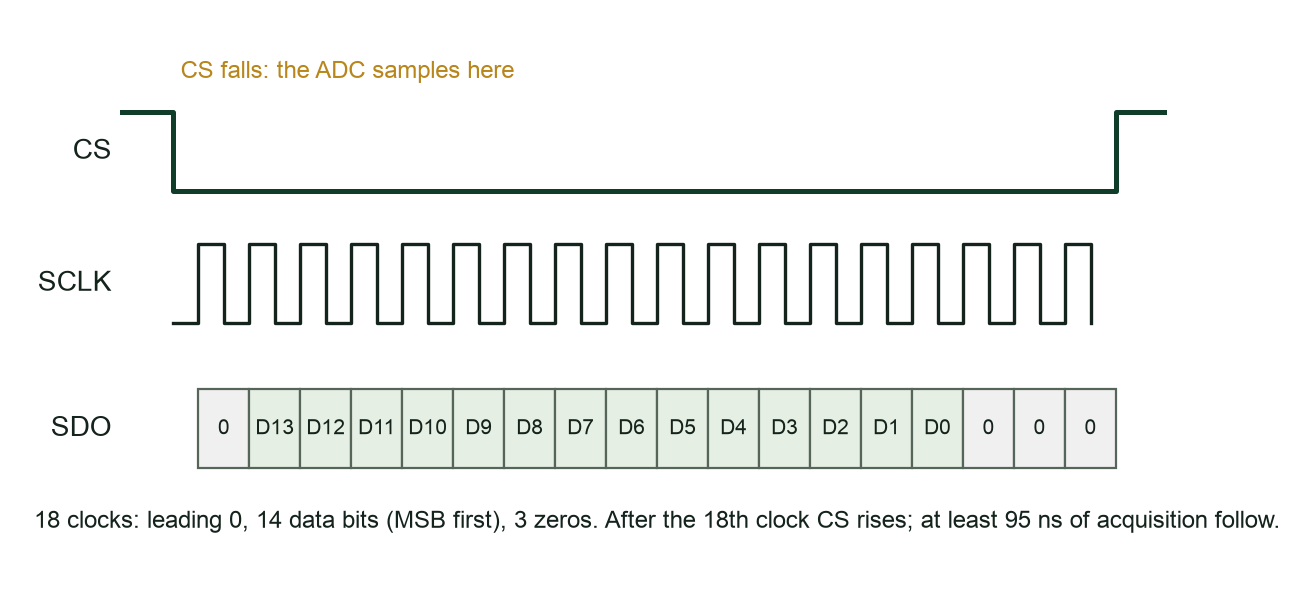
\includegraphics[width=0.56\textwidth]{fig_spi.png}
\caption{One frame. CS falls and the ADC samples. After 18 clocks, CS rises and the ADC acquires for at least 95 ns.}\label{fig:spi}
\end{figure}
\begin{pass}CS, SCLK, and SDO agree with Figure~\ref{fig:spi}. The first frame returns zeros. Each next frame returns the sample of the frame before.\end{pass}
\begin{fail}If all data is zero, read the data twice, because the data comes one frame late. If SDO is stuck, check +3V3 at pin 4 of U4 and R18 to R20 (22 $\Omega$).\end{fail}
\end{samepage}

% ---------------- Step 7
\clearpage
\begin{samepage}
\stepno{7}{The ADC codes}
\goal{make sure the codes follow the input.}
\begin{enumerate}
\item Apply no signal to J1. Read 4096 samples. Calculate the mean (offset) and the rms noise in codes. One code is 0.403 mV.
\item Apply a sine of 100 mV peak at 250 kHz at SIG\_IN. Read 4096 samples. Find the peak code.
\item Increase SCLK to 20 MHz, then to 25 MHz. Look for errors in the samples.
\item If the samples have errors, move the sample edge of the host later.
\end{enumerate}
\begin{table}[H]
\caption{Expected codes.}
\small\begin{tabular}{@{}lll@{}}
\toprule Test & Expected & Limit\\\midrule
First frame (24 clocks) & all zeros & -\\
Offset with the input idle & about 0 codes & $\pm$10 codes\\
Noise with the input idle (no sensor) & about 1 code rms (estimate) & below 3 codes\\
Peak for 100 mV at SIG\_IN and 250 kHz & $\pm$1018 codes & $\pm$10\,\%\\
Sample rate at 10, 20, 25, and 60 MHz & 0.53, 1.01, 1.23, and 2.50 MSPS & -\\
\bottomrule\end{tabular}
\end{table}
\begin{pass}The codes follow the input in size and sign. SCLK at 25 MHz gives no errors. The idle noise is below 3 codes.\end{pass}
\begin{fail}If the word is wrong, remember the format: one leading zero, 14 data bits (D13 first, two's complement), and three zeros. If the offset is large, check VOCM at \tp{14} and VMID5 at \tp{13}.\end{fail}
\end{samepage}

% ---------------- Step 7
\clearpage
\begin{samepage}
\stepno{8}{The sensor head alone}
\goal{make sure the charge amplifier converts charge to voltage with the gain Q/Cf.}
The head (10 $\times$ 27 mm) gets power through the coax from SENSOR IN. Close JP1 on the main board. Connect an SMA cable from J6 of the head to J1.
\begin{figure}[H]
\centering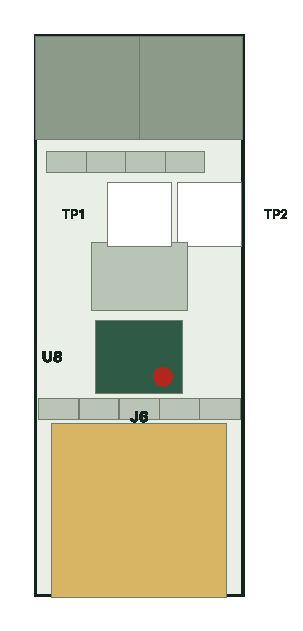
\includegraphics[height=4.4cm]{fig_headmap.pdf}\hfill
\parbox[b]{9.6cm}{\small\textbf{Head connections}\\[2pt]\begin{tabular}{@{}ll@{}}\texttt{TP1} (+) & piezo $+$ pad (summing node)\\\texttt{TP2} ($-$) & piezo $-$ pad (head ground)\\J6 & SMA to J1 of the main board\\U8 & OPA365, pin 1 as in Step 0\\\end{tabular}}
\caption{The sensor head. The two large holes at the top are the M2 mounting holes.}
\end{figure}
\begin{enumerate}
\item Wait 25 s. The reference divider (two 1 M$\Omega$ resistors and 10 $\mu$F) needs this time to settle.
\item Measure the DC voltage at the head. The pad of C37 must be about 2.9 V. The pad of C35 must be about 1.45 V.
\item Make sure the supply current is about 4.3 mA higher than in Step 1.
\item Connect the generator through a 10 pF C0G capacitor to \texttt{TP1}. Connect the generator ground to \texttt{TP2}.
\item Set the generator to a burst of 10 cycles at 250 kHz.
\item Read the peak at \tp{3} on the main board for each row of Table~\ref{tab:head}.
\item Stop the generator. Connect the 1600 pF C0G capacitor between \texttt{TP1} and \texttt{TP2} as a dummy sensor.
\item Record \tp{6} with the input quiet. The noise gain is 35, as with the real sensor.
\end{enumerate}
\begin{table}[H]
\caption{Expected head output for Cf = 47 pF and Q = 10 pF $\times$ V. The tolerance is $\pm$10\,\%.}\label{tab:head}
\small\begin{tabular}{@{}rrrrl@{}}
\toprule Generator (peak) & Charge & Head output at \tp{3} & \tp{6} (chain) & Listener\\\midrule
100 mV & 1 pC & 21 mV & 87 mV & no change\\
300 mV & 3 pC & 64 mV & 262 mV & WAKE\_N falls\\
1000 mV & 10 pC & 213 mV & 874 mV & both fall\\
\bottomrule\end{tabular}
\end{table}
\begin{pass}Each output is within 10\,\% of Table~\ref{tab:head}. A real event of 4 to 7 pC gives 85 to 149 mV. WAKE\_N falls for each event, and BIG\_N falls above 5.2 pC. The noise at the ADC with the dummy sensor is below 2 codes. The simulation gives 0.2 codes.\end{pass}
\begin{fail}If there is no output, make sure JP1 is closed and the head has DC power. If the DC voltage is wrong, check pin 1 of U8, R29, and R30. If the gain is wrong, check C34 (47 pF C0G) and R28 (1 M$\Omega$). If the noise is very high with the dummy sensor, wait 25 s. Then check the coax and the ground.\end{fail}
\end{samepage}

% ---------------- Step 8, 9
\clearpage
\begin{samepage}
\stepno{9}{The head and the board together}
\goal{make sure one full chain works from the head connector to the ZedBoard.}
\begin{enumerate}
\item Connect the head to J1 with the coax. Leave JP1 closed.
\item Power the board from the PMOD.
\item Inject 3 pC as in Step 8 while the ZedBoard reads the ADC.
\item Find the peak code.
\item Make sure WAKE\_N falls for the length of the burst.
\end{enumerate}
\begin{pass}The peak code is about 650. This value is 262 mV divided by 0.403 mV. WAKE\_N falls for the length of the burst.\end{pass}
\bigskip
\stepno{10}{The sensor on the plant}
\goal{make the first real recording.}
\begin{enumerate}
\item Solder the piezo sensor to the head.
\item Mount the sensor on the plant.
\item Record a window that is long enough for several events.
\item Compare the peak frequency and the amplitude with the perfboard results. The old data has peaks at 233 to 275 kHz and charges of 4 to 7 pC.
\item Note the rms noise in codes.
\item Note the highest frequency in an event.
\end{enumerate}
The two last numbers help the next design.
\end{samepage}

% ---------------- troubleshooting
\clearpage
\section{Troubleshooting}
Start at the top of Figure~\ref{fig:flow}. Find the first question with the answer no. Look only at that stage.
\begin{figure}[H]
\centering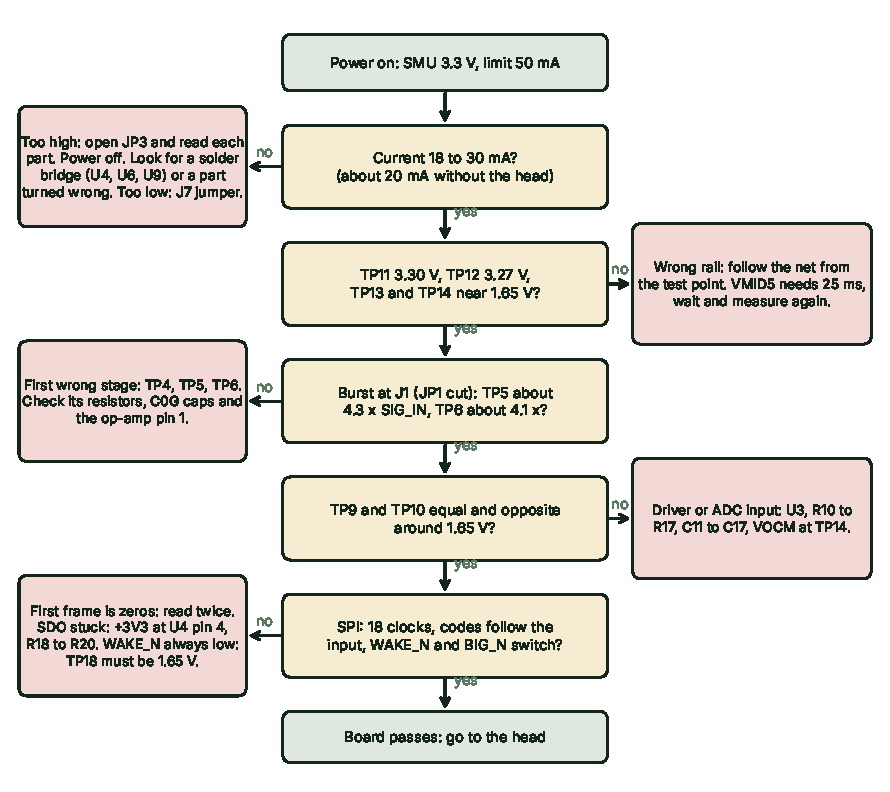
\includegraphics[width=\textwidth]{fig_flow.pdf}
\caption{Decision chart for the main board.}\label{fig:flow}
\end{figure}

% ---------------- record
\clearpage
\section{Record sheet}
Write the readings in the table. Board serial: \rule{3cm}{0.3pt}\quad Date: \rule{3cm}{0.3pt}\quad Power: $\square$ SMU $\square$ PMOD

\small\begin{tabular}{@{}p{4.6cm}p{3.1cm}p{2.6cm}p{2.2cm}p{1.2cm}@{}}
\toprule Check & Expected & Measured & Limit & OK\\\midrule
\tp{11} to \tp{19} resistance & about 2 k$\Omega$ & & $>$ 1 k$\Omega$ & \\
Supply current (no head) & 20 to 22 mA & & 18 to 30 mA & \\
+3V3 (\tp{11}) & 3.30 V & & $\pm$30 mV & \\
AVDD (\tp{12}) & 3.27 V & & $\pm$50 mV & \\
VMID5 (\tp{13}) & 1.65 V & & $\pm$50 mV & \\
VOCM (\tp{14}) & 1.64 V & & $\pm$50 mV & \\
REFL (\tp{18}) & 1.64 V & & $\pm$50 mV & \\
\tp{5} / \tp{3} at 250 kHz & 4.29 & & $\pm$10 \% & \\
\tp{6} / \tp{3} at 250 kHz & 4.10 & & $\pm$10 \% & \\
\tp{7}, \tp{8} (each, 100 mV in) & $\pm$205 mV & & $\pm$10 \% & \\
Gain at 100 / 500 kHz (dB) & $-3.1$ / $-2.8$ & & $\pm$1.5 dB & \\
WAKE\_N threshold & 35 mV & & $\pm$12 mV & \\
BIG\_N threshold & 111 mV & & $\pm$12 mV & \\
ADC offset (codes) & 0 & & $\pm$10 & \\
ADC noise, input idle (codes rms) & about 1 & & $<$ 3 & \\
Peak code for 100 mV at 250 kHz & 1018 & & $\pm$10 \% & \\
Head: DC at C37 / C35 & 2.9 V / 1.45 V & & $\pm$0.1 V & \\
Head: 3 pC at \tp{3} & 64 mV & & $\pm$10 \% & \\
\bottomrule\end{tabular}

\normalsize
\subsection*{Notes}
\rule{\textwidth}{0.3pt}\\[10pt]\rule{\textwidth}{0.3pt}\\[10pt]\rule{\textwidth}{0.3pt}\\[10pt]\rule{\textwidth}{0.3pt}
\end{document}
